% Figure M5 hero prototype : generated by experiments/m5_vit_cls.py --hero.
% Preview-only; not yet linked from the main manuscript.
\begin{figure}[t]
 \centering
 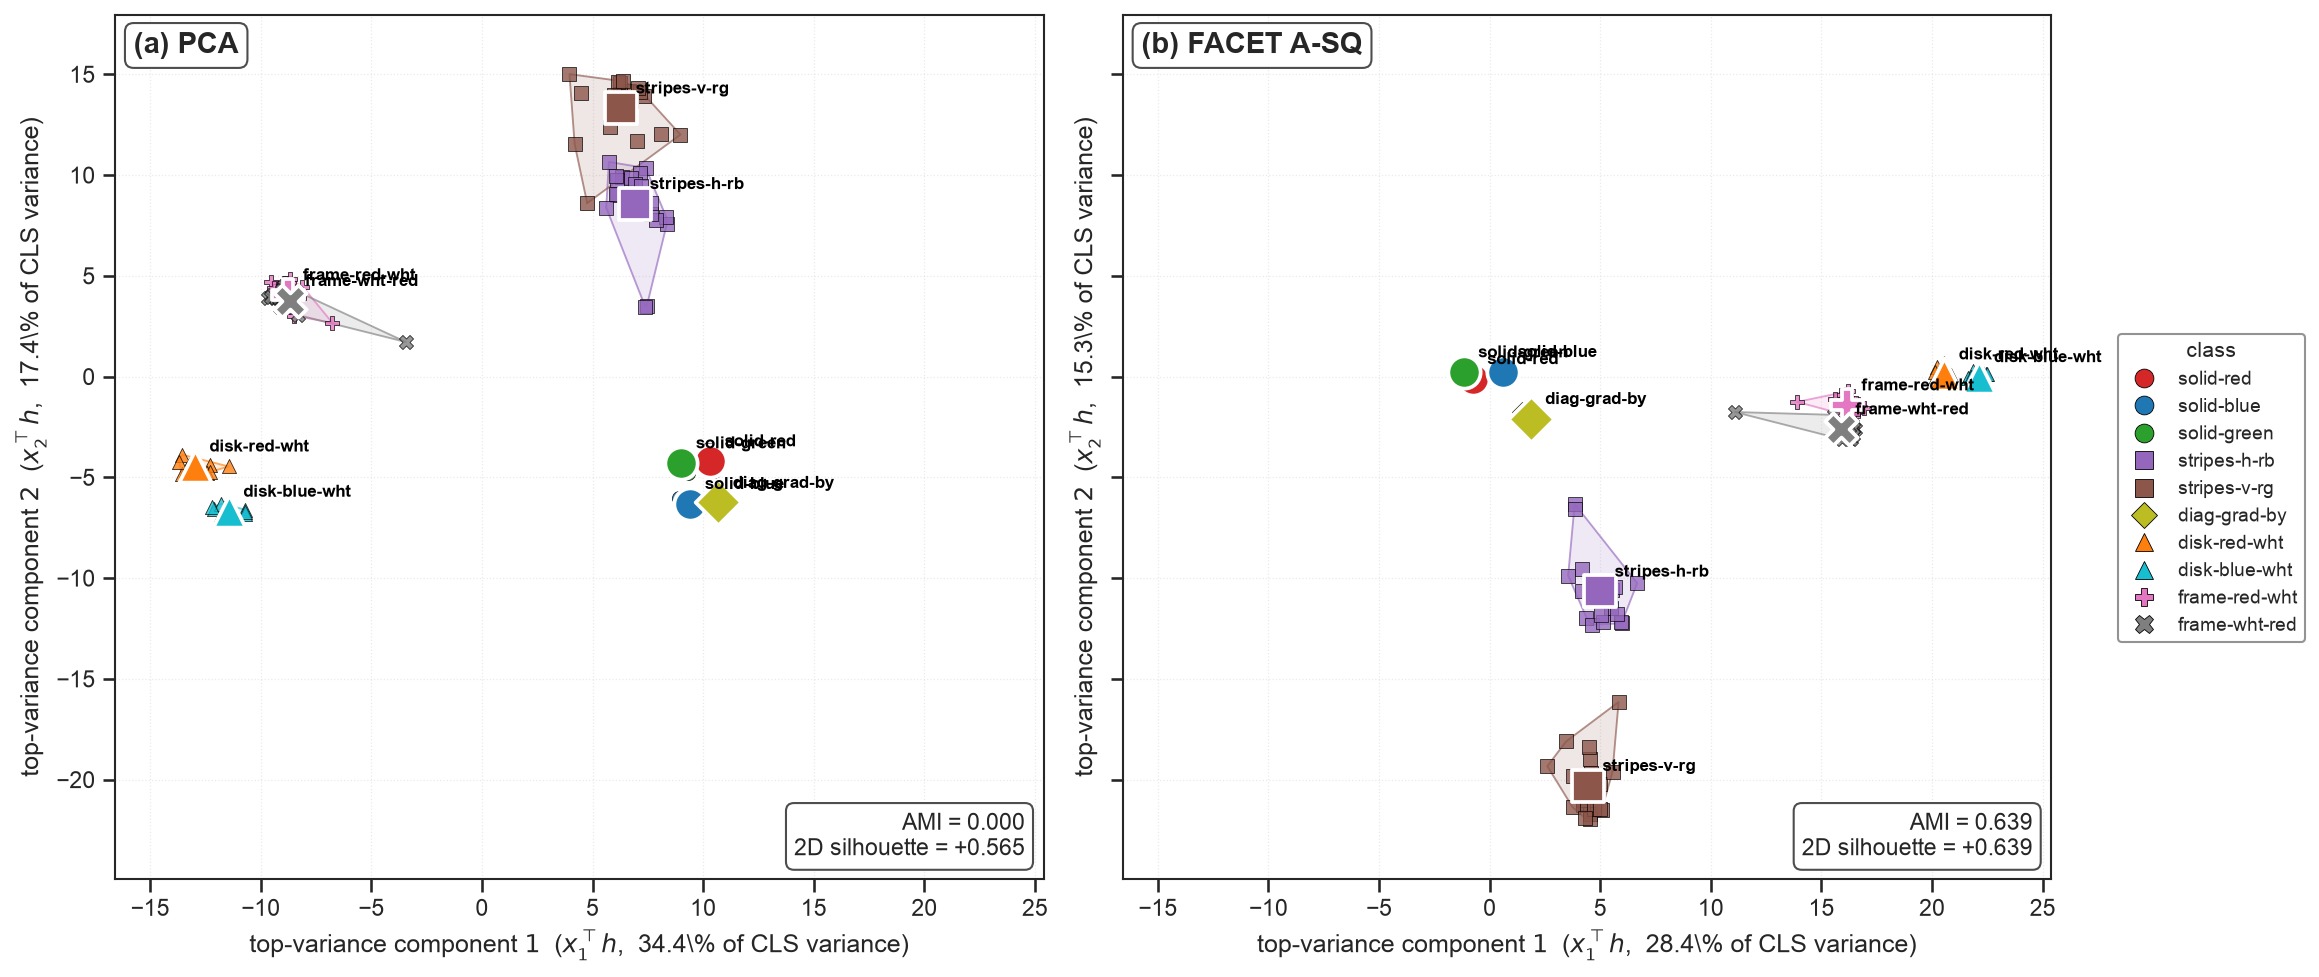
\includegraphics[width=\linewidth]{../shared/figures/generated/m5_vit_cls_hero.png}
 \caption{\textbf{M5 hero: the AMI gap in two dimensions.} Each ViT-base CLS token projected onto its own method's two variance-dominant components at matched $m{=}10$ on the same $200$-image synthetic set ($10$ classes $\times$ $20$ variants). Markers are coloured by ground-truth class; the large labelled X-markers are per-class centroids. Both panels share axis limits so cluster spread is directly comparable. In-panel badges report the dominant-component AMI against the ground-truth labels. \textbf{(a)}~Under PCA the ten class centroids pile into the centre of the plane and the point clouds overlap; the dominant-component partition is uncorrelated with class, AMI $\approx 0$. \textbf{(b)}~Under FACET A-SQ the ten centroids separate into visibly disjoint clusters covering the plane, matching AMI $=0.639$. Both decompositions achieve $R^2\approx 0.968$ on the same CLS token set, so the clustering difference comes entirely from the threshold operator forcing class-conditional specialisation of the components (Theorem~\ref{thm:identification}).}
 \label{fig:m5-vit-cls-hero}
\end{figure}
